\documentclass[12pt, a4paper]{report}

\usepackage{graphicx}               %inclusão de figuras
\usepackage[caption=false]{subfig}  %permite o uso do comando subfloat
\usepackage{amsmath, amssymb}       %inclusão de símbolos matemáticos 
\usepackage{lmodern}                %habilita alguns caracteres latinos extras
\usepackage[T1]{fontenc}            %permite acentuação
\usepackage[utf8]{inputenc}         %idem anterior - no windows usar latin1
\usepackage[brazil,brazilian]{babel}%habilita hifenizações
\usepackage{cite}                   %converte [1,2,3,4,5] -> [1-5]
\usepackage[margin= 2.5cm]{geometry}%define o tamanho das margens
\usepackage[normalem]{ulem}         %permite sublinhar uma palavra
\usepackage{setspace}               %permite usar espaçamento \onehalfspacing \doublespacing
\usepackage{indentfirst}            %indenta o primeiro parágrafo
\usepackage{color, colortbl}        %permite textos e tabelas coloridas
\usepackage{booktabs, array}        %comandos adicionais para melhorar a qualidade das tabelas
\usepackage{multirow}               %permite juntar linhas de uma tabela
\usepackage{appendix}               %aumenta alguns recursos de \appendix
\usepackage{hyperref}               %gera hiperlinks no pdf
	\hypersetup{colorlinks, citecolor=blue, linkcolor=blue, urlcolor=blue} 

\newcommand{\sen}{\operatorname{sen}}

\begin{document}

%capa
% capa
\begin{titlepage}
	\begin{center}
		\setstretch{2.0}
		\begin{tabular}{m{4cm}m{10cm}}
			\multirow{3}{*}{\vspace{-0.5cm}
\includegraphics[width=2.8cm]{fig/uem}}
			& {\LARGE Universidade Estadual de Maringá} \\
			& {\LARGE Centro de Ciências Exatas} \\
			& {\LARGE Departamento de Física} \\
		\end{tabular}
		\vspace{1.8cm}
	
		{\LARGE Trabalho de Conclusão de Curso | Dissertação | Tese}
		\vspace{4.0cm}

		{\LARGE {\bf Título do trabalho de conclusão de curso
ou dissertação ou tese}}
		\vfill

		\setstretch{1}	
		{\Large Acadêmico: Fulando da Silva}
		\vspace{0.8cm}
	
		{\Large Orientador: Prof. Dr. Ciclano da Silva}
		\vspace{1.2cm}
		
		{\large Maringá, \today}
	\end{center}
\end{titlepage}

% página de rosto
\begin{titlepage}
	\begin{center}
		\setstretch{2.0}
		\begin{tabular}{m{4cm}m{10cm}}
			\multirow{3}{*}{\vspace{-0.5cm}
\includegraphics[width=2.8cm]{fig/uem}}
			& {\LARGE Universidade Estadual de Maringá} \\
			& {\LARGE Centro de Ciências Exatas} \\
			& {\LARGE Departamento de Física} \\
		\end{tabular}
		\vspace{1.8cm}
	
		{\LARGE Trabalho de Conclusão de Curso | Dissertação | Tese}
		\vspace{4.0cm}

		{\LARGE {\bf Título do trabalho de conclusão de curso
ou dissertação ou tese}}
		\vfill

		\setstretch{1}	
		\hspace*{7.0cm}\parbox{9.0cm}
		{\large Tese ao Departamento de
Física da Universidade Estadual de Maringá, sob orientação do professor
Dr. Ciclano da Silda, como parte dos requisitos para obtenção do título
de Doutor em Física}
		\vfill
	
		{\Large Acadêmico: Fulando da Silva}
		\vspace{0.8cm}
	
		{\Large Orientador: Prof. Dr. Ciclano da Silva}
		\vspace{1.2cm}
	
		{\large Maringá, \today}
	\end{center}
\end{titlepage}


\pagenumbering{roman}

%sumário
\tableofcontents

%agradecimentos
\chapter*{Agradecimentos}
\addcontentsline{toc}{chapter}{Agradecimentos}

Meu sinceros agradecimentos ao prof. Dr. Ciclano da Silva pela
orientação.

À Capes, ao CNPq e à Fundação Araucária pelo suporte financeiro. 

E por último, mas não menos importante, gostaria de agradecer minha
família pelo apoio contínuo.


%resumo
\chapter*{Resumo}
\addcontentsline{toc}{chapter}{Resumo}

Neste trabalho estudamos... 
\vspace{1.5cm}

{\bf Palavras chave:} física, matéria condensada, cosmologia.


%abstract
\chapter*{Abstract}
\addcontentsline{toc}{chapter}{Abstract}

In this work we study... 
\vspace{1.5cm}

{\bf Keywords:} phisycs, condensed matter, cosmology.


\pagenumbering{arabic}

%introdução
\chapter*{Introdução}
\addcontentsline{toc}{chapter}{Introdução}

Uma breve introdução sobre o tema que será abordado na tese. Veja como
usar uma citação de um livro \cite{Butkov_book}, notas de aula
\cite{Rosas}, tese de doutorado \cite{simeao_phdthesis}, dissertação de
mestrado \cite{oliveira_mastersthesis}, patente \cite{fernandes_pat},
e-mails \cite{manuel} e artigos \cite{B1, B2, A1, A2, A3}.

No \hyperlink{cap1}{capítulo 1} abordaremos ... No
\hyperlink{cap2}{capítulo 2} o assunto tal será tratado... Por fim, são
apresentadas algumas \hyperlink{conc}{conclusões}, discussões e
perspectivas futuras


%capítulos
\hypertarget{cap1}{}
\chapter{Título do capítulo 1}

Escrever brevemente sobre o que será abordado nesse capítulo.

\section{Título da seção}

As figuras \ref{s-01} e \ref{s-02} mostram a distribuição de um
conjunto de moléculas formando a fase nemática uniaxial. Apesar de
ambas possuírem a mesma direção orientacional, definida pelo diretor,
$\vec{n}$, existe uma visível diferença no grau de ordenamento entre
elas.
\begin{figure}[!htb]
	\centering
	\subfloat[]{\label{s-01}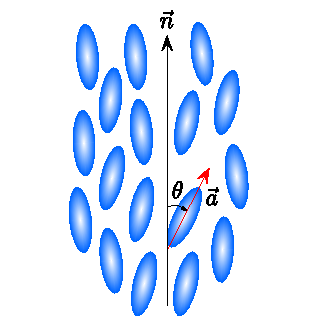
\includegraphics[scale= 1.0]{fig/s-01}}
	\hspace{1cm}
	\subfloat[]{\label{s-02}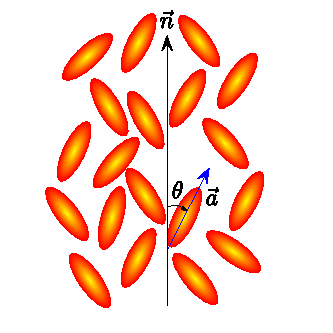
\includegraphics[scale= 1.0]{fig/s-02}}
	\caption{As figuras apresentam mesma direção orientacional,
contudo diferentes graus de ordenamento. Podemos observar que a figura
(a) possui uma menor dispersão da média, definida pelo diretor,
do que a figura (b).}
	\label{fig1}
\end{figure}

Este grau de alinhamento pode ser descrito por uma função
distribuição normalizada\footnote{$\oint f(\theta)\, d\Omega =
\int_{0}^{2\pi} \int_{0}^{\pi} f(\theta)\, {\rm sen}\, \theta\,
d\theta\, d\phi = 1$}, $f(\theta)\, d\theta$, que fornece a
probabilidade de encontrar o eixo principal de uma molécula, $\vec{a}$,
formando um ângulo entre $\theta$ e $\theta + d\theta$ com o diretor.
Devido à simetria cilíndrica das moléculas, a função distribuição
é independente do ângulo azimutal, $\phi$.

O parâmetro de ordem tensorial $Q_{ij}$ pode ser representado por uma
matriz, ou seja,
\begin{equation*} 
	Q_{ij}=\left(
		\begin{array}{ccc} 
			-(S + P)/2 & 0          & 0\\ 
			0          & -(S - P)/2 & 0\\ 
			0          & 0          & S
		\end{array}\right)\ ,
\end{equation*}
onde $S$ e $P$ são os parâmetros de ordem escalares. A equação
\eqref{eq2} mostra como fazer uma equação dentro de uma caixa
\begin{equation}
	\boxed{\Tilde{\mathcal{F}}_{\rm LdG}= \frac{\sigma}{2} \, {\rm
Tr}\Tilde{\bf Q}^2 - {\rm Tr}\Tilde{\bf Q}^3 + \frac{1}{2}\, ({\rm
Tr}\Tilde{\bf Q}^2)^2 + ... }\ .
	\label{eq2}
\end{equation}

Não esqueça de ver o \hyperlink{apen}{Apêndice A}.

\hypertarget{cap2}{}
\chapter{Resultados}

Os parâmetros que utilizaremos nas simulações estão listados na tabela
\ref{tabela}.
\begin{table}[!htb]
	\begin{minipage}[b]{0.49\linewidth}
	  \begin{center}
	    \begin{tabular}{c l l}
	\multicolumn{3}{l}{MBBA} \\ 
	\hline 
	\hline 
	$a$               & $= \, 0,0867 \times 10^{6}$   & ${\rm J/Km}^{3}$ \\
	$B$               & $= \, -2,12  \times 10^{6}$   & ${\rm J/m}^{3}$  \\
	$C$               & $= \, 1,74   \times 10^{6}$   & ${\rm J/m}^{3}$  \\
	$\mathcal{L}1$    & $= \, 6,93   \times 10^{-12}$ & ${\rm N}$        \\
	$\mathcal{L}2$    & $= \, 0,0    \times 10^{-12}$ & ${\rm N}$        \\
	$(T-T^{*})$       & $= \, (307,0- 311,0)$         & ${\rm K}$        \\
	$\Delta$          & $= \, 1,0    \times 10^{-9}$  & ${\rm m}$        \\
	$\Delta t$        & $= \, 3,5    \times 10^{-9}$  & ${\rm s}$        \\
	$\mu_1$           & $= \, 0,2 $                   & ${\rm Pa\, s}$   \\
	$\Delta \epsilon$ & $= \, -0,6$                   &                  \\
	$S_{\rm eq}$      & $= \, 0,62$                   &                  \\
	\hline
	    \end{tabular}
	  \end{center}
	\end{minipage}
	\begin{minipage}[b]{0.49\linewidth}
	  \begin{center}
	    \begin{tabular}{c l l}
	\multicolumn{3}{l}{5CB} \\ 
	\hline
	\hline 
	$a$               & $= \, 0,14  \times 10^{6}$   & ${\rm J/Km}^{3}$ \\
	$B$               & $= \, -1,80 \times 10^{6}$   & ${\rm J/m}^{3}$  \\
	$C$               & $= \, 3,60  \times 10^{6}$   & ${\rm J/m}^{3}$  \\
	$\mathcal{L}1$    & $= \, 3,0   \times 10^{-12}$ & ${\rm N}$        \\
	$\mathcal{L}2$    & $= \, 0,0   \times 10^{-12}$ & ${\rm N}$        \\
	$(T-T^{*})$       & $= \, (298,0- 307,2)$        & ${\rm K}$        \\
	$\Delta$          & $= \, 1,0   \times 10^{-9}$  & ${\rm m}$        \\
	$\Delta t$        & $= \, 15    \times 10^{-9}$  & ${\rm s}$        \\
	$\mu_1$           & $= \, 0,3 $                  & ${\rm Pa\, s}$   \\
	$\Delta \epsilon$ & $= \, 11,5$                  &                  \\
	$S_{\rm eq}$      & $= \, 0,58$                  &                  \\
	\hline
	    \end{tabular}
	  \end{center}
	\end{minipage}
	\caption{{\small Parâmetros dos cristais líquidos
MBBA (4-methoxybenzylidene-4-butylanaline) e 5CB
(4-cyano-4'-pentylbiphenyl).}}
	\label{tabela}
\end{table}

A tabela \ref{tabela1} mostra como destacar algumas partes da tabela.
\begin{table}[!htb]
  \begin{center}
    \begin{tabular}{ l | c | c | c }
& $\Delta =0,9 {\rm nm}$ & $\Delta =1,0 {\rm nm}$ & $\Delta =1,5 {\rm
nm}$ \\
		\hline
$\Gamma =1$ & $0,409\pm 0,004$ & \cellcolor[gray]{0.9} $0,412\pm 0,004$
& $0,409\pm 0,009$ \\
		\hline
$\Gamma =\frac{1}{(1-{\rm Tr}{\bf Q}^2)^2}$ & \cellcolor[gray]{0.9}
$0,413\pm 0,004$ & $0,409\pm 0,002$ & $0,406\pm 0,009$ \\
		\hline
    \end{tabular}
  \end{center}
\caption{Comparação entre os expoentes $\alpha$ obtidos pelo
ajuste dos dados de uma média de $100$ condições iniciais de uma rede
de $256 \times 256$ utilizando a lei de potências, $L(t) \varpropto
t^{\alpha}$.}
	\label{tabela1}
\end{table}

Veja as figuras \ref{figura-1} e \ref{figura-2}. Também observe a figura
\ref{MBBA-3}.

\begin{figure}[!htb]
  \centering
		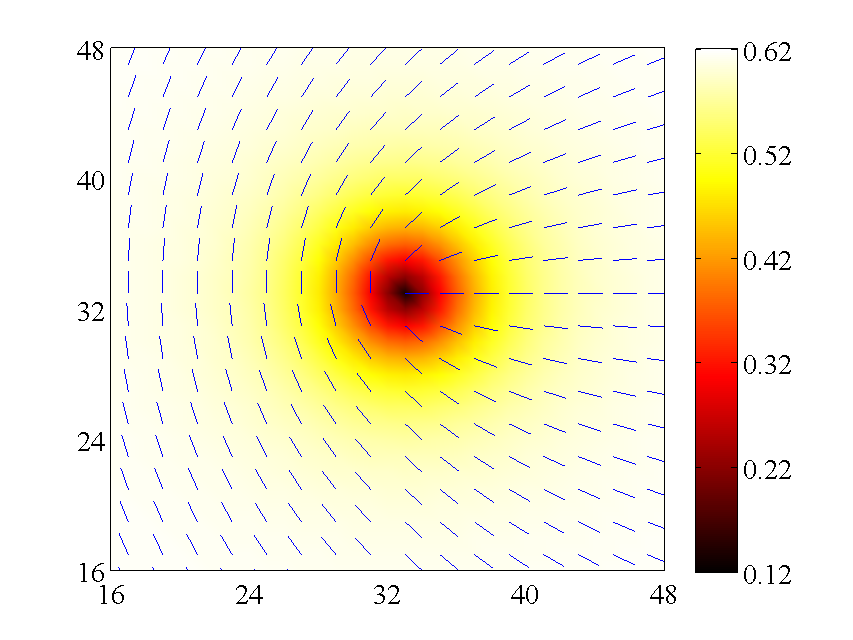
\includegraphics[width= 7.0cm]{fig/fig-1}
  \caption{A figura mostra o perfil de $S$ junto com a projeção do
diretor no plano $x-y$}
  \label{figura-1}
\end{figure}

\begin{figure}[!htb]
  \centering
		\subfloat[$t= 0$  ]{\label{MBBA-1}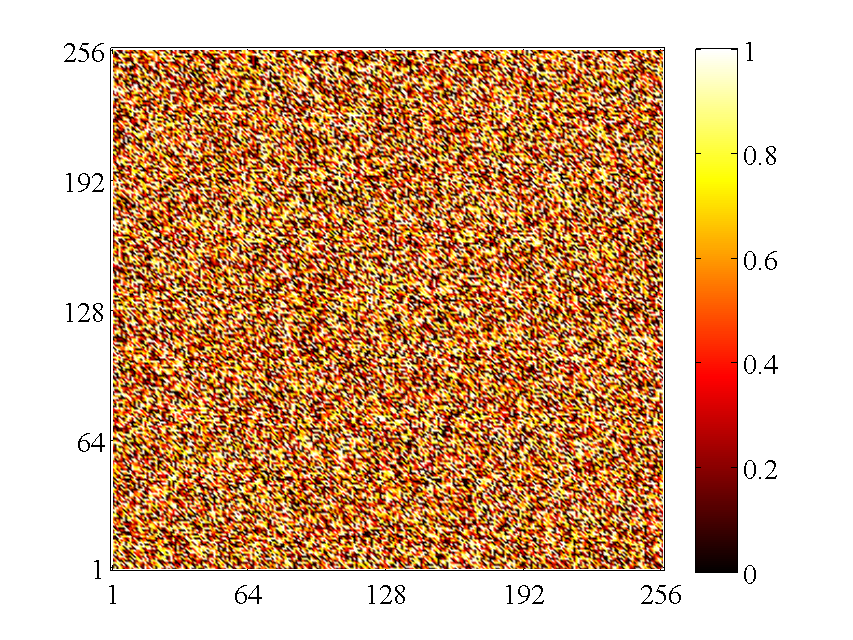
\includegraphics[scale= 0.55]{fig/MBBA-1}}
		\subfloat[$t= 2$  ]{\label{MBBA-2}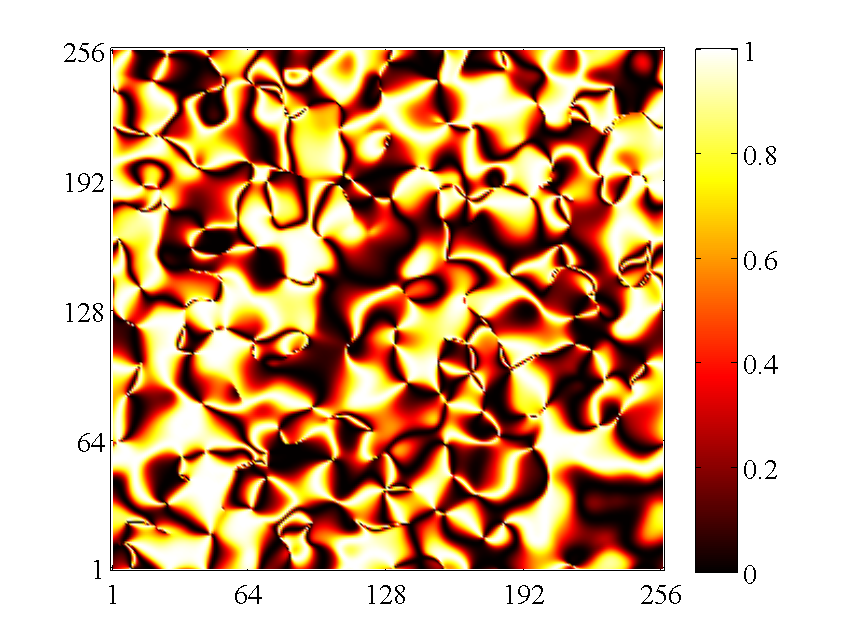
\includegraphics[scale= 0.55]{fig/MBBA-2}}
		\\
		\subfloat[$t= 20$ ]{\label{MBBA-3}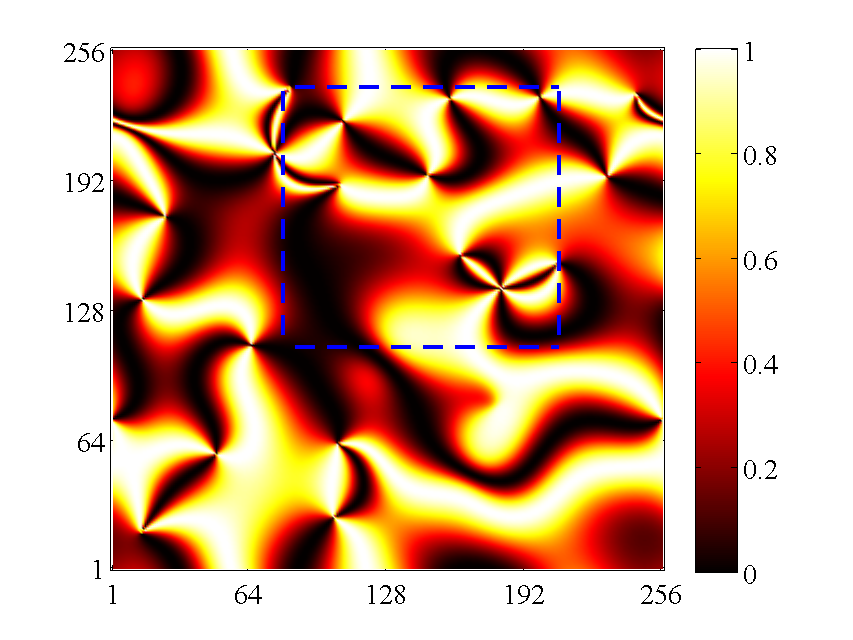
\includegraphics[scale= 0.55]{fig/MBBA-3}}
		\subfloat[$t= 200$]{\label{MBBA-4}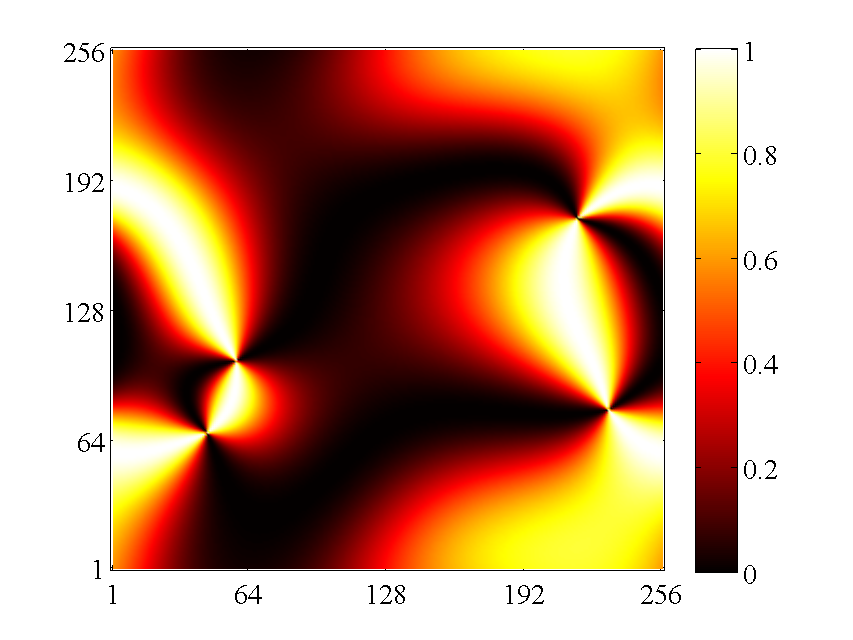
\includegraphics[scale= 0.55]{fig/MBBA-4}}
  \caption{Nesta sequência temporal de imagens é mostrado o valor
do ${\rm sen}^2(2\beta)$ em cada ponto da rede, onde $\beta$ é o ângulo
que o diretor forma com o eixo do polarizador que, neste caso, coincide
com o eixo horizontal.}
  \label{figura-2}
\end{figure}


%conclusão
\chapter*{Conclusões}
\addcontentsline{toc}{chapter}{Conclusões}
\hypertarget{conc}{}

Neste trabalho abordamos sobre...

Entre as perspectivas de trabalhos futuros, pretendemos...


%apêndices
\appendix
\hypertarget{apen}{}
\chapter{Contas e mais contas}

Como discutido no \hyperlink{cap1}{Capítulo 1}, a equação que rege a
dinâmica de orientação do diretor no volume de um cristal líquido
nemático é dada por

\begin{eqnarray}
\frac{1}{\Lambda} \frac{\partial}{\partial \Tilde{t}} \Tilde{Q}_{ij} & =
& - \Gamma_{ijkl} \left[ \frac{\partial \Tilde{\mathcal{F}}_{\rm
LdG}}{\partial \Tilde{Q}_{kl}}- \frac{\partial }{\partial
\Tilde{x}_m}\frac{\partial \Tilde{\mathcal{F}}_{\rm LdG}}{\partial
\Tilde{Q}_{kl,\Tilde{m}}}\right] -\Gamma_{ijkl} \left[ \frac{\partial
\Tilde{\mathcal{F}}_{\rm el}}{\partial \Tilde{Q}_{kl}}- \frac{\partial
}{\partial \Tilde{x}_m}\frac{\partial \Tilde{\mathcal{F}}_{\rm
el}}{\partial \Tilde{Q}_{kl,\Tilde{m}}}\right] \nonumber \\ & &
\nonumber \\ & & -\Gamma_{ijkl}\left[ \frac{\partial
\Tilde{\mathcal{F}}_{\rm E}}{\partial \Tilde{Q}_{kl}}- \frac{\partial
}{\partial \Tilde{x}_m}\frac{\partial \Tilde{\mathcal{F}}_{\rm
E}}{\partial \Tilde{Q}_{kl,\Tilde{m}}}\right]\,,
	\label{dinamica_volume} 
\end{eqnarray}
onde, como já foi visto, $\Lambda= 2B^2 \Delta t / 9C^2\mu_1$,
$\Gamma_{ijkl}= ( \frac{1}{2} \delta_{ik} \delta_{jl}+ \frac{1}{2}
\delta_{il} \delta_{jk}- \frac{1}{3} \delta_{ij} \delta_{kl})$,
$\Tilde{t}= t/\Delta t$, $\Tilde{x}_m = x_m/\Delta$, e
$\Tilde{\mathcal{F}}_{\rm LdG}$, $\Tilde{\mathcal{F}}_{\rm el}$ e
$\Tilde{\mathcal{F}}_{\rm E}$ são as densidades de energia de Landau-de
Gennes, elástica e de um campo elétrico externo, respectivamente.


%bibliográfia
\newpage
\phantomsection \label{bibliography}
\addcontentsline{toc}{chapter}{Referências Bibliográficas}
\bibliographystyle{ieeetr}
\bibliography{tese}

\end{document}
